\documentclass[11pt,a4paper]{article}
\usepackage[utf8]{inputenc}
\usepackage[T1]{fontenc}
\usepackage{lmodern}
\usepackage[a4paper,margin=2.2cm]{geometry}
\usepackage{setspace}\onehalfspacing
\setlength{\parskip}{0.4em}\setlength{\parindent}{1.2em}
\usepackage{amsmath,amssymb}
\usepackage{booktabs,tabularx,array}
\renewcommand{\arraystretch}{1.2}
\usepackage{graphicx}
\usepackage[shortlabels]{enumitem}
\usepackage{fancyhdr}
\pagestyle{fancy}\fancyhf{}
\fancyhead[L]{\small\textsc{Mineração de Séries Temporais} -- Atividade da Aula 1}
\fancyhead[R]{\small\thepage}
\renewcommand{\headrulewidth}{0.4pt}
\usepackage[hidelinks]{hyperref}
\usepackage[most]{tcolorbox}
\newtcolorbox{resposta}[1][]{enhanced,breakable,colback=white,colframe=black,boxrule=0.5pt,leftrule=3pt,arc=0pt,outer arc=0pt,fonttitle=\bfseries\small,title=Resposta,#1}
\renewcommand{\figurename}{Figura}\renewcommand{\tablename}{Tabela}

\title{\bfseries Atividade da Aula 1 -- Análise da série temporal PETR4}
\author{César Willian Pacheco\\ \small Especialização em Inteligência Artificial \& Ciência de Dados -- PUCPR\\ \small Prof.\ Vinícius Mourão Alves de Souza}
\date{Setembro de 2026}

\begin{document}
\maketitle
\thispagestyle{fancy}

\section*{Enunciado e dados}
Analise a série temporal da Petrobras (\texttt{PETR4.csv}) disponibilizada: (i) a série é univariada ou multivariada? (ii) qual a taxa de amostragem? (iii) qual a dimensionalidade em termos de variáveis e quantidade de observações? (iv) em qual data a série apresentou o maior valor de fechamento (\textit{Close}) e qual foi esse valor? (v) em relação às séries \textit{Close} e \textit{Volume}, o que se pode afirmar sobre tendência, ciclo, sazonalidade, autocorrelação e estacionariedade?

O arquivo do professor (\texttt{gdown 1vUh6gxcfFeKreamBk3JKS7QsAmRS8ME5}) contém cotações diárias de PETR4.SA no formato do Yahoo Finance, de 02/01/2020 a 30/12/2025. Como o CSV não estava na pasta local, a série foi reconstruída a partir da mesma fonte (API do Yahoo Finance, mesmo ticker e período); os valores de abertura, fechamento e volume conferem com os do arquivo do professor nas linhas verificadas (o arquivo do Yahoo traz 1494 pregões; o CSV do professor, 1493 -- falta o pregão de 06/01/2020). Todos os números abaixo foram produzidos pelo script \texttt{analise\_petr4.py} (pandas, statsmodels, scipy), anexo.

\section{Univariada ou multivariada?}
\begin{resposta}
\textbf{Multivariada.} Em cada instante (pregão) são registradas simultaneamente cinco variáveis: \texttt{Open}, \texttt{High}, \texttt{Low}, \texttt{Close} e \texttt{Volume} -- exatamente o exemplo ``Ações (open, close, low, high, volume)'' dos slides. A quantidade de variáveis observadas ao mesmo tempo é o que define o caráter multivariado, e não o número de observações. A atividade, porém, pede a análise de \textit{Close} e \textit{Volume} \textbf{separadamente}: é a estratégia mencionada em aula de tratar cada canal como uma série \textbf{univariada} independente, o que permite aplicar as técnicas univariadas (média móvel, decomposição, ACF, testes de estacionariedade) ao custo de ignorar a relação entre os canais (por exemplo, o volume tende a disparar nos dias de queda brusca do preço).
\end{resposta}

\section{Taxa de amostragem}
\begin{resposta}
\textbf{Uma observação por dia útil de pregão da B3} (frequência diária, intervalo \emph{regular no calendário de negociação}, mas irregular no calendário civil). Entre observações consecutivas o intervalo é de 1 dia em 1153 casos, 3 dias em 286 (fins de semana), e de 2, 4 ou 5 dias em 54 casos (feriados). Não há observações em sábados ou domingos e há 70 dias úteis sem pregão (feriados da bolsa). Na média, são \textbf{249,3 observações por ano} (248 a 251 por ano civil), o que justifica usar $m \approx 252$ como período anual nas análises sazonais. A hora ``16:56:00'' presente nas datas do CSV é apenas o horário de captura da cotação de fechamento e não indica amostragem intradiária.
\end{resposta}

\begin{figure}[h]\centering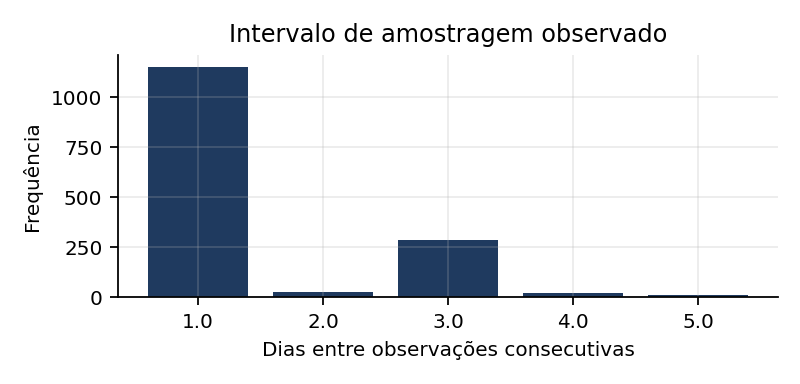
\includegraphics[width=0.55\linewidth]{figuras/intervalo_amostragem.png}
\caption{Distribuição dos intervalos (em dias corridos) entre observações consecutivas.}\end{figure}

\section{Dimensionalidade}
\begin{resposta}
\textbf{5 variáveis $\times$ 1494 observações} (matriz $1494 \times 5$), cobrindo 02/01/2020 a 30/12/2025 (seis anos civis). No arquivo original do professor há 1493 linhas, pela ausência de um pregão. Considerando somente as séries analisadas, cada uma (\textit{Close} e \textit{Volume}) é um vetor de comprimento $n = 1494$.
\end{resposta}

\section{Maior valor de fechamento}
\begin{resposta}
O maior fechamento ocorreu em \textbf{19/02/2024}, com \textbf{Close = R\$~42,90}. Para referência, o menor fechamento foi R\$~11,29 em 18/03/2020, no auge da queda provocada pela pandemia e pela guerra de preços do petróleo.
\end{resposta}

\begin{figure}[h]\centering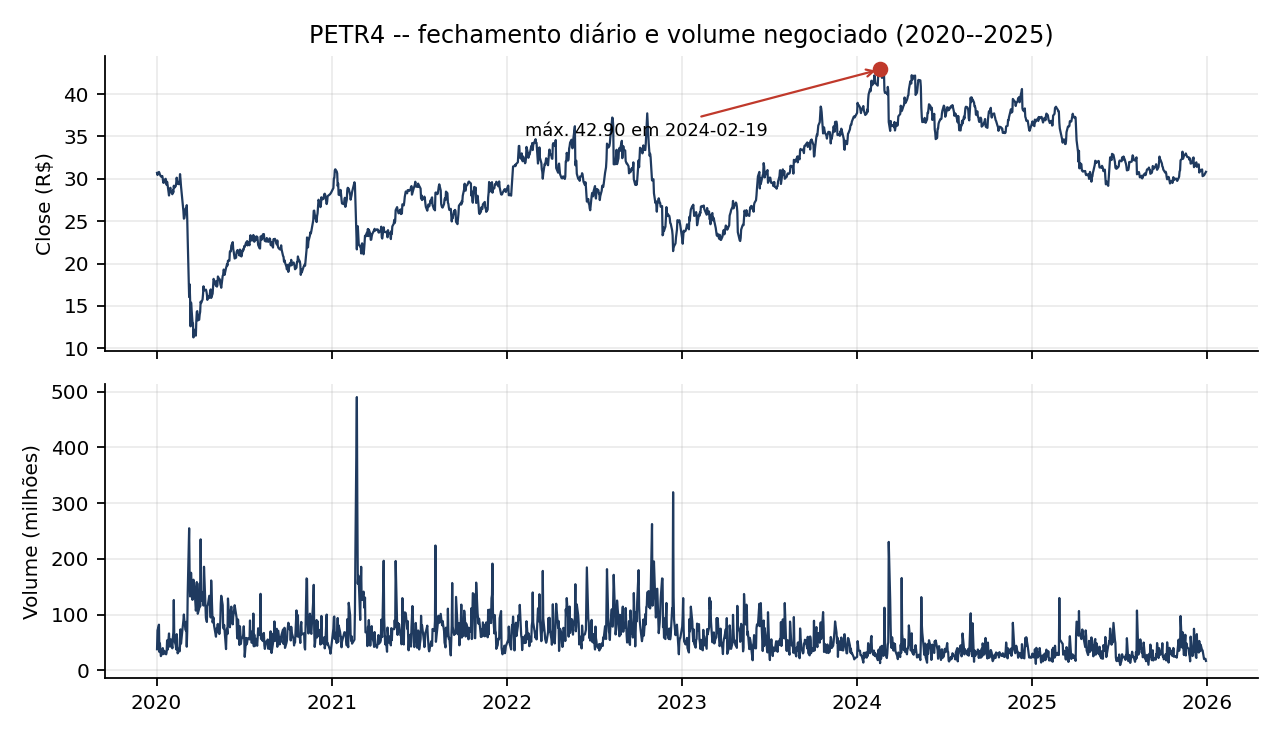
\includegraphics[width=0.95\linewidth]{figuras/visao_geral.png}
\caption{Fechamento diário e volume negociado de PETR4 (2020--2025); o ponto marca o maior fechamento.}\end{figure}

\section{Características das séries \textit{Close} e \textit{Volume}}

\subsection*{Resumo quantitativo}
\begin{center}\small
\begin{tabularx}{\linewidth}{@{}l X X@{}}
\toprule
\textbf{Característica} & \textbf{Close (R\$)} & \textbf{Volume (ações/dia)} \\
\midrule
Médias anuais & 22,3 (2020); 26,9 (2021); 30,7 (2022); 29,7 (2023); 38,2 (2024); 32,7 (2025) & 75,3 M (2020); 79,1 M (2021); 82,3 M (2022); 57,2 M (2023); 37,1 M (2024); 35,1 M (2025) \\
Variação início$\to$fim & $+0{,}4\%$ (30,70 $\to$ 30,82) & $-55\%$ (37,8 M $\to$ 16,9 M) \\
Picos da série suavizada (ciclos) & set/2022 e mar/2024 (375 pregões entre eles) & abr/2020, abr/2021, out/2021, nov/2022 (234, 139 e 256 pregões) \\
Amplitude do componente sazonal anual & 4,64 (15\% da média); força sazonal 0,19 & $1{,}2\times10^{8}$; força sazonal 0,25 \\
ACF lag 1 / 5 / 21 / 252 & 0,993 / 0,963 / 0,849 / 0,165 & 0,639 / 0,426 / 0,271 / 0,159 \\
ACF da 1ª diferença (lag 1) & 0,000 & $-0{,}312$ \\
ADF ($H_0$: raiz unitária), $p$ & 0,153 (não rejeita) & $1{,}0\times10^{-5}$ (rejeita) \\
KPSS ($H_0$: estacionária), $p$ & 0,01 (rejeita) & 0,01 (rejeita) \\
Média/desvio em 5 janelas & 23,0/4,7; 28,7/3,1; 28,1/3,5; 37,1/2,7; 33,6/3,0 & 79,6/46,6; 74,5/29,4; 74,9/36,3; 41,4/22,5; 34,9/17,2 (milhões) \\
\bottomrule
\end{tabularx}
\end{center}
\noindent Limite de significância aproximado da ACF: $\pm 1{,}96/\sqrt{1494} = \pm 0{,}051$.

\subsection*{Tendência}
\begin{resposta}
\textbf{Close:} não há uma direção única de longo prazo. A média móvel de 126 pregões mostra uma \emph{tendência não monotônica}: queda abrupta no 1º trimestre de 2020, recuperação e alta até 2022, recuo em 2022--início de 2023, forte alta até o pico de 2024 e queda em 2025. Como a série termina praticamente no mesmo nível em que começou ($+0{,}4\%$), a regressão linear global tem inclinação quase nula ($\approx 0{,}01$ R\$/pregão); a tendência é \emph{local}, como no exemplo da taxa de desemprego visto em aula.\\
\textbf{Volume:} tendência de longo prazo \textbf{decrescente}: as médias anuais caem de $\approx 80$ milhões de ações/dia em 2020--2022 para $\approx 35$ milhões em 2024--2025 ($-55\%$ ponta a ponta), com o volume mais alto concentrado nos períodos de crise (março de 2020) e de forte volatilidade.
\end{resposta}

\begin{figure}[h]\centering
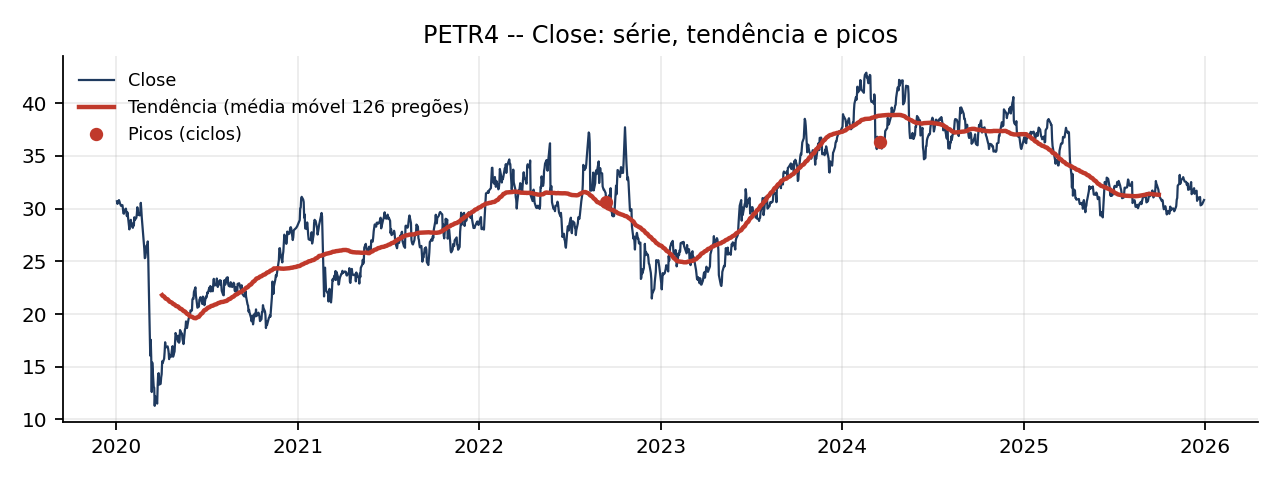
\includegraphics[width=0.95\linewidth]{figuras/close_tendencia.png}\\[2pt]
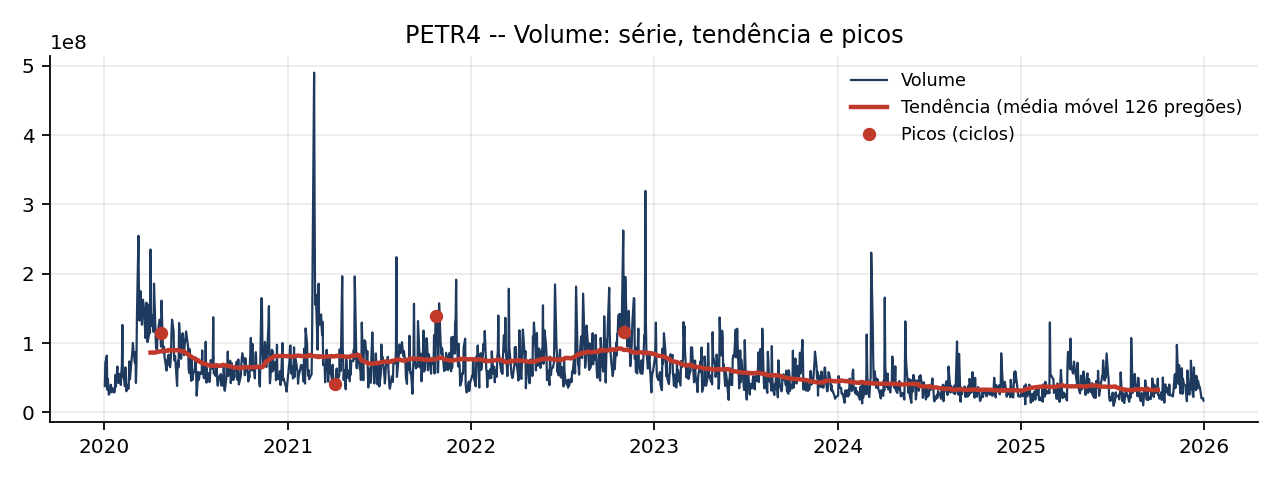
\includegraphics[width=0.95\linewidth]{figuras/volume_tendencia.png}
\caption{Séries com a tendência (média móvel centrada de 126 pregões) e os picos relevantes da versão suavizada.}\end{figure}

\subsection*{Ciclos}
\begin{resposta}
Ambas apresentam \textbf{oscilações de longo prazo com duração irregular} -- o que os slides definem como ciclo, distinto de sazonalidade. Aplicando ao \textit{Close} suavizado (média móvel de 63 pregões) a detecção de picos por proeminência, como no notebook do professor, obtêm-se picos em set/2022 e mar/2024, separados por 375 pregões ($\approx 1{,}5$ ano); visualmente há ainda os vales de mar/2020 e mar/2023. Esses ciclos correspondem a ciclos econômicos e do preço do petróleo (pandemia, recuperação, guerra na Ucrânia, política de dividendos e preços da empresa) e não a um calendário fixo. No \textit{Volume} os picos (abr/2020, abr/2021, out/2021, nov/2022) estão a 234, 139 e 256 pregões uns dos outros, também sem período constante: são episódios de estresse do mercado, não ciclos regulares.
\end{resposta}

\subsection*{Sazonalidade}
\begin{resposta}
\textbf{Não há sazonalidade relevante em nenhuma das duas séries.} Na decomposição aditiva com período anual ($m = 252$), o componente sazonal do \textit{Close} tem amplitude de 4,6 (15\% da média) mas força sazonal de apenas 0,19: o componente que o método extrai é irregular, com amplitude menor do que a do resíduo (desvio 2,15), e não se repete de forma reconhecível ano a ano -- é o mesmo ``falso positivo'' do contraexemplo da temperatura horária discutido em aula: \texttt{seasonal\_decompose} sempre devolve algum padrão, cabe ao analista julgar se ele é real. A ACF no lag anual (252) é baixa (0,16 para \textit{Close}, 0,16 para \textit{Volume}) e não apresenta o pico que caracteriza séries sazonais como a temperatura (0,79 no lag 365) ou a demanda por bicicletas (picos em 24 e 168 horas). Também não há efeito de dia da semana: as médias de \textit{Close} por dia da semana variam entre 30,02 e 30,17, e as de \textit{Volume} sobem suavemente de segunda (58 M) a sexta (66 M) -- um efeito de calendário fraco, que não configura um padrão sazonal definido. Isso é esperado em preços de ações: um padrão sazonal previsível seria rapidamente arbitrado pelo mercado.
\end{resposta}

\begin{figure}[h]\centering
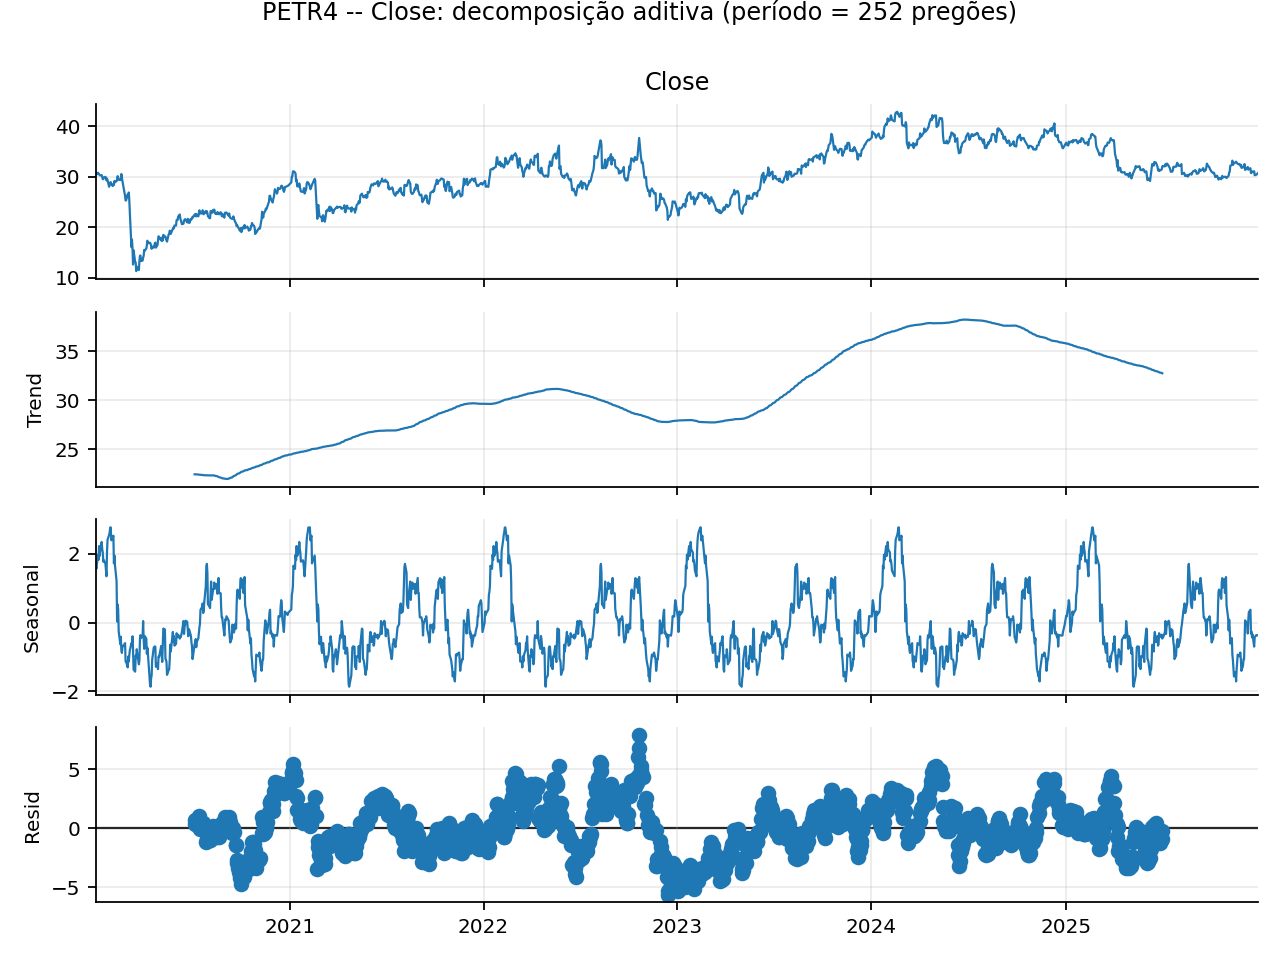
\includegraphics[width=0.49\linewidth]{figuras/close_decomposicao.png}
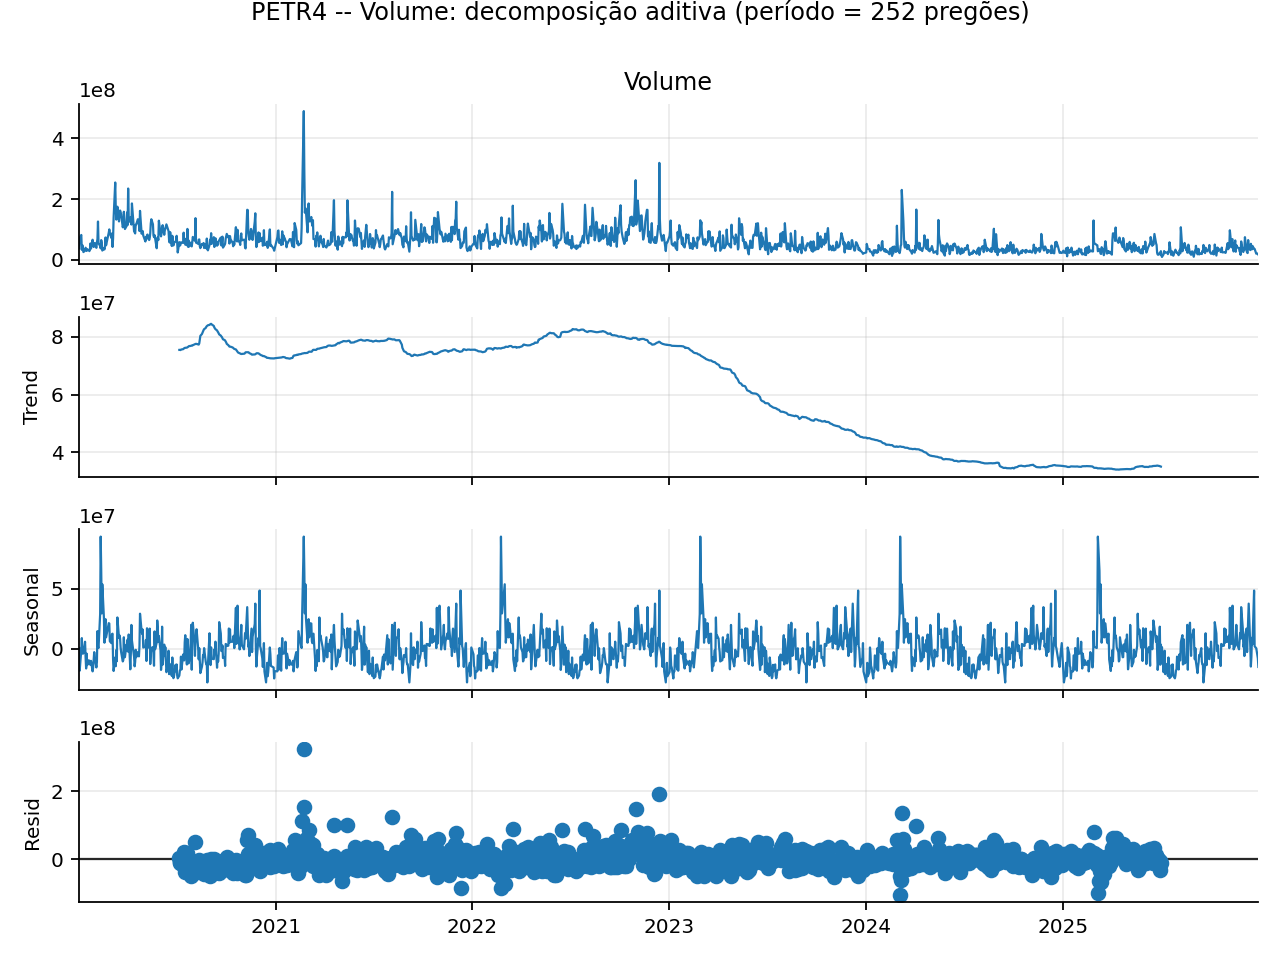
\includegraphics[width=0.49\linewidth]{figuras/volume_decomposicao.png}
\caption{Decomposição aditiva (tendência, sazonalidade anual e resíduo) de \textit{Close} e \textit{Volume}.}\end{figure}

\subsection*{Autocorrelação}
\begin{resposta}
\textbf{Close:} autocorrelação \textbf{muito forte e persistente}: $\rho(1) = 0{,}993$, $\rho(5) = 0{,}963$, $\rho(21) = 0{,}849$, $\rho(63) = 0{,}669$, com decaimento lento e aproximadamente linear da ACF -- assinatura típica de um passeio aleatório (raiz unitária). A PACF corta após o lag 1, o que indica que praticamente toda a dependência é explicada pelo valor do dia anterior. O passado ``ajuda a responder o presente'' apenas no sentido de que o preço de hoje é a melhor estimativa do de amanhã: a ACF da \emph{primeira diferença} (retornos) é nula em todos os lags ($\rho(1) = 0{,}000$), ou seja, as variações diárias não são previsíveis linearmente a partir das variações passadas.\\
\textbf{Volume:} autocorrelação \textbf{moderada e de decaimento rápido}: $\rho(1) = 0{,}64$, $\rho(5) = 0{,}43$, $\rho(21) = 0{,}27$, estabilizando em torno de 0,15--0,25 para lags longos (efeito da tendência decrescente). Dias de volume alto tendem a ser seguidos por dias de volume alto (\emph{agrupamento} de atividade), mas a memória é curta. A ACF da diferença é negativa no lag 1 ($-0{,}31$), sinal de reversão à média: um salto de volume tende a ser parcialmente desfeito no dia seguinte.
\end{resposta}

\begin{figure}[h]\centering
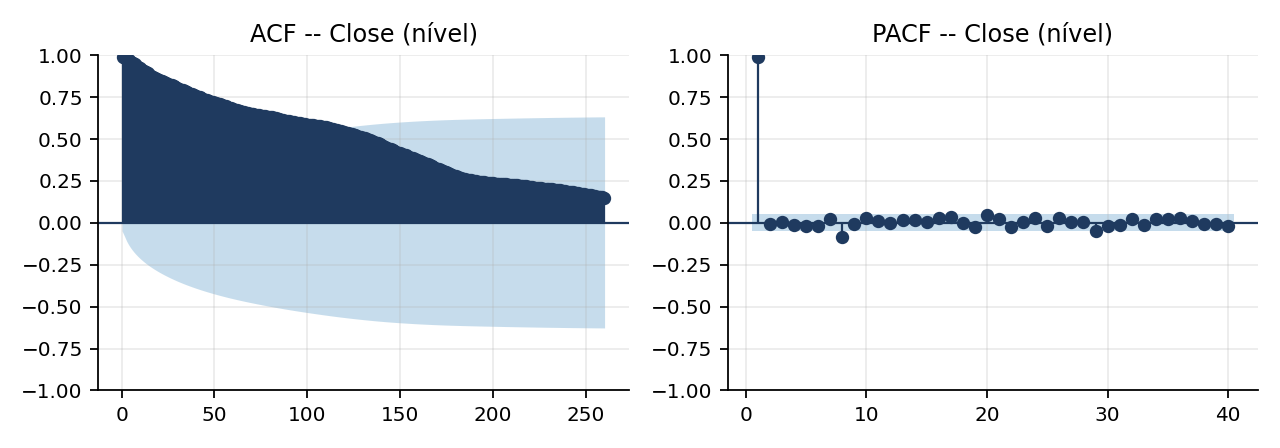
\includegraphics[width=0.95\linewidth]{figuras/close_acf_pacf.png}\\[2pt]
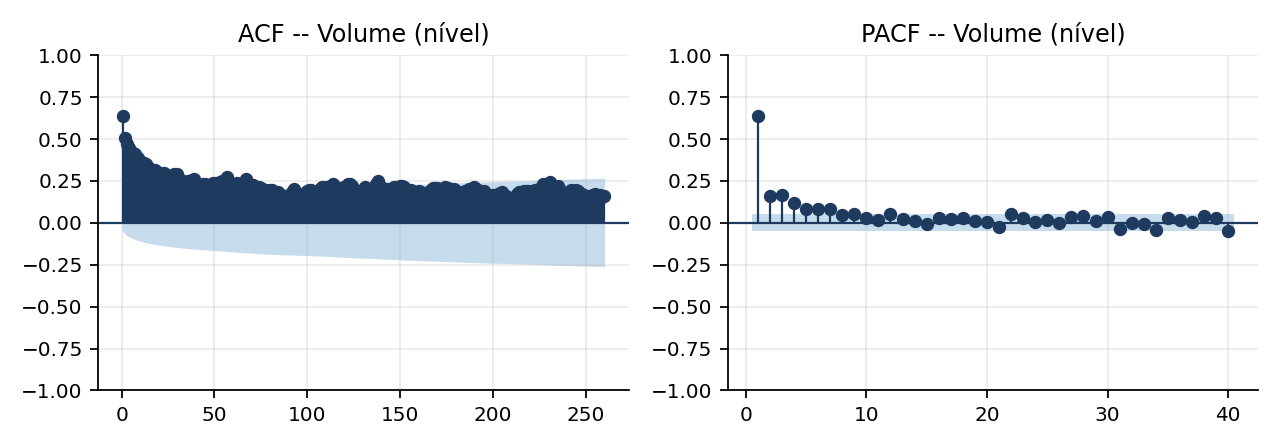
\includegraphics[width=0.95\linewidth]{figuras/volume_acf_pacf.png}
\caption{ACF (até 260 lags) e PACF (40 lags) das séries em nível; a faixa azul é o intervalo de confiança de 95\%.}\end{figure}

\subsection*{Estacionariedade}
\begin{resposta}
\textbf{Close: não estacionária.} O teste ADF não rejeita a hipótese de raiz unitária ($p = 0{,}153$) e o KPSS rejeita a hipótese de estacionariedade ($p = 0{,}01$); os dois testes concordam. As estatísticas por janela confirmam: a média passa de 23,0 para 37,1 entre a 1ª e a 4ª janela e o desvio-padrão varia de 2,7 a 4,7. A \emph{primeira diferença}, porém, é estacionária (ADF $p < 10^{-10}$; KPSS $p = 0{,}10$, não rejeita) -- a série é integrada de ordem 1, $I(1)$, o que justifica o componente ``I'' com $d = 1$ de um modelo ARIMA, tema da Aula 2.\\
\textbf{Volume: não estacionária, mas por razão diferente.} O ADF rejeita a raiz unitária ($p \approx 10^{-5}$): não há passeio aleatório, a série oscila em torno de um nível. Entretanto o KPSS também rejeita a estacionariedade ($p = 0{,}01$), porque esse nível \emph{muda} ao longo do tempo (tendência decrescente: médias por janela de 79,6 M para 34,9 M) e a variância também cai (desvio de 46,6 M para 17,2 M). Trata-se de \emph{não estacionariedade em tendência e em variância}, tratável por diferenciação ou por transformação logarítmica seguida de remoção da tendência. A divergência entre ADF e KPSS é justamente o caso em que a série é ``estacionária em torno de uma tendência'', e ilustra por que os slides recomendam olhar as estatísticas em janelas além dos testes.
\end{resposta}

\begin{figure}[h]\centering
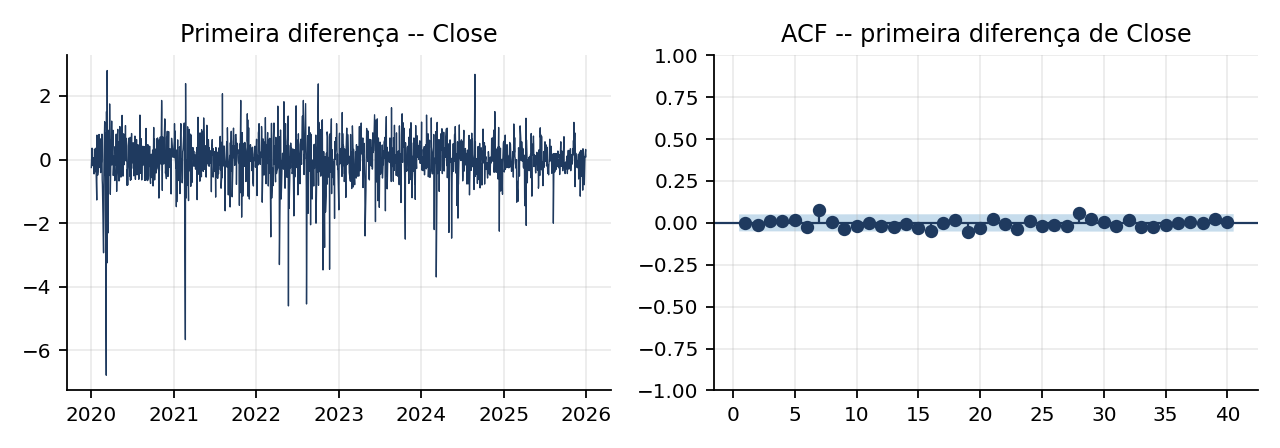
\includegraphics[width=0.95\linewidth]{figuras/close_diferenca.png}\\[2pt]
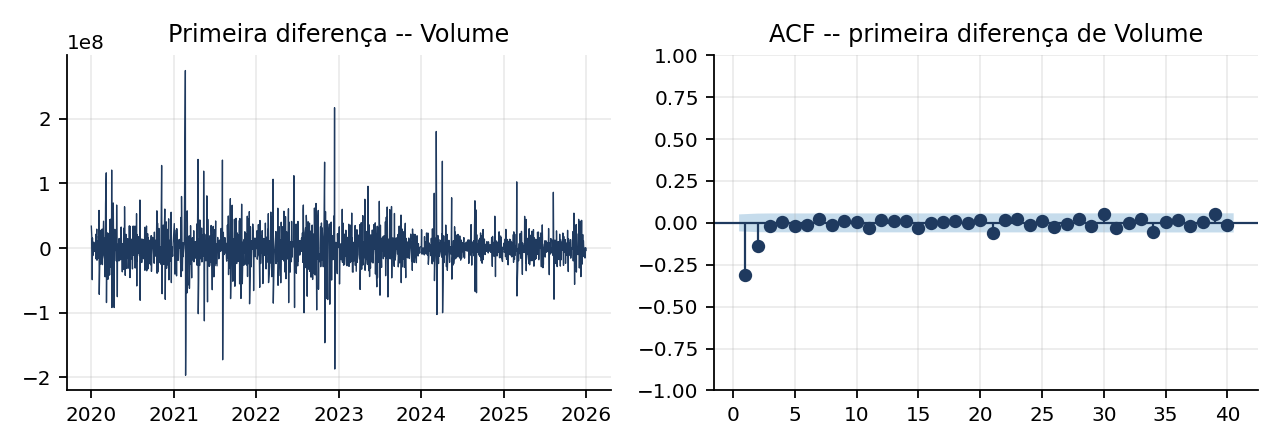
\includegraphics[width=0.95\linewidth]{figuras/volume_diferenca.png}
\caption{Primeira diferença das séries e sua ACF: os retornos de \textit{Close} não têm autocorrelação; a diferença do \textit{Volume} apresenta reversão à média (lag 1 negativo).}\end{figure}

\section*{Síntese}
A série PETR4 é multivariada (5 variáveis $\times$ 1494 pregões, uma observação por dia útil), com fechamento máximo de R\$~42,90 em 19/02/2024. O \textit{Close} é um processo altamente autocorrelacionado, não estacionário (raiz unitária), com tendência local não monotônica, ciclos irregulares de origem econômica e sem sazonalidade; sua primeira diferença é ruído sem memória. O \textit{Volume} tem tendência decrescente, memória curta, reversão à média, ciclos ligados a episódios de estresse do mercado e também não apresenta sazonalidade. Essas conclusões orientam a Aula 2: para o preço, baselines \emph{naive} (último valor) e modelos com diferenciação (ARIMA com $d = 1$) são pontos de partida naturais; para o volume, modelos que capturem nível variável e memória curta.

\vspace{0.5em}\noindent\small\textit{Arquivos entregues:} \texttt{analise\_petr4.py} (script completo), \texttt{PETR4.csv}, \texttt{resultados.json} e a pasta \texttt{figuras/}.
\end{document}
